\documentclass[10pt,twocolumn,letterpaper]{article}
\usepackage[review]{cvpr}
\usepackage{graphicx}
\usepackage{booktabs}
\usepackage{amsmath,amssymb}
\usepackage{multirow}
\usepackage{xcolor}
\usepackage{url}
\usepackage{microtype}
\graphicspath{{figures/}}

\definecolor{cvprblue}{rgb}{0.21,0.49,0.74}
\usepackage[pagebackref,breaklinks,colorlinks,allcolors=cvprblue]{hyperref}
\def\paperID{*****}
\def\confName{CVPR}
\def\confYear{2026}
\title{Supplementary Material: From Measurement Overlap to Shared Influence}

\begin{document}
\maketitle

\section{Scope and Audit Contract}
This supplement expands experiments already reported in the main paper; it does not introduce a tuned or corrected method. All reliability scores use only information available from acquired anchors or already generated reconstructions. Dense targets are evaluation-only. The independent units are 24 fastMRI examinations, 115 IXI examinations, and eight NingXia patients containing 22 series. Whenever NingXia series are resampled, the patient prefix is the cluster and all subordinate series move together. Unless noted, intervals use 5,000 examination/patient-cluster bootstrap replicates.

The principal Plan6 tests were registered before their corresponding outputs were computed. The neural influence stage gate was evaluated on one central plane, then expanded without changing seeds, perturbation size, endpoints, contexts, or statistical rules. The IXI $\times2$ checkpoint, SHA-256, mask, endpoint, and budgets were frozen before any test output existed. All negative results in Sec.~\ref{sec:negative} remain in the evidence record.

\paragraph{Cohort and endpoint accounting.}
Frozen HAT and SwinIR $\times4$ reconstructions exist for all three cohorts. fastMRI and NingXia have same-program $\times2$ outcomes; IXI $\times2$ was produced by a separately frozen I3Net checkpoint, so the IXI benefit experiment is explicitly cross-estimator. Every examination score is reduced before cohort ranking, preventing long volumes from contributing more statistical weight.

\begin{table*}[t]
\centering
\caption{Analysis units and frozen neural-influence coverage.}
\label{tab:s_cohorts}
\setlength{\tabcolsep}{7pt}
\begin{tabular}{lrrrr}
\toprule
Cohort&Cases/series&Clusters&Planes/model&Models\\
\midrule
fastMRI&24&24&72&HAT, SwinIR\\
IXI&115&115&345&HAT, SwinIR\\
NingXia&22&8&66&HAT, SwinIR\\
\bottomrule
\end{tabular}
\end{table*}

\section{Definitions and Frozen Neural Perturbation}
For two context-specific target errors $e_a,e_b$, define
\begin{align}
E_{\rm pair}&=\tfrac12(\|e_a\|_2^2+\|e_b\|_2^2),\\
E_{\rm shared}&=\|\tfrac12(e_a+e_b)\|_2^2,\\
E_{\rm obs}&=\|\tfrac12(e_a-e_b)\|_2^2.
\end{align}
The shared and observable fractions are $E_{\rm shared}/E_{\rm pair}$ and $E_{\rm obs}/E_{\rm pair}$, respectively; they sum to one up to floating-point error. Prediction squared disagreement equals $4E_{\rm obs}$. Error cosine is computed on the common foreground support. These are paired reconstruction-error quantities, not posterior uncertainty.

For each physical anchor shared by contexts $a,b$, the same centered Rademacher field $\xi_{js}$ is added to both context inputs at one percent of the globally normalized case range. With frozen network $F_c$,
\begin{equation}
r_{cjs}=F_c(x+\epsilon\xi_{js})-F_c(x).
\end{equation}
The reported neural shared influence averages the cosine between $r_{ajs}$ and $r_{bjs}$ over common anchors and seeds 6101--6104. Each field is centered within the evaluation support. The perturbation is deterministic given case, plane, anchor, and seed. No target image is used to compute the influence score. Common response mass is retained as a magnitude-aware secondary definition.

\paragraph{Controlled context grid.}
The reference context uses offsets $(-2,+2)$ around a physically matched target. Eight non-self comparator contexts retain two input anchors and vary overlap, span, asymmetry, and anchor identity. Target, model, preprocessing, foreground support, and input count are fixed. Broad-grid partial ranks residualize examination, overlap, span, and asymmetry. A stricter four-context subset fixes overlap count at exactly one and residualizes examination, span, and asymmetry; count itself cannot explain variation in this subset.

\section{Full Neural Shared-Influence Results}
Table~\ref{tab:s_neural} reports every architecture stratum for the three primary paired-error endpoints. Neural influence improves absolute association over count in all 18 comparisons. Every clustered interval for the advantage excludes zero. Conditional associations after removing the measured geometry labels remain nonzero in the expected direction ($|\rho|=0.185$--$0.395$). Thus the result is not only a re-expression of integer overlap, although unmeasured context properties can remain.

\begin{table*}[t]
\centering
\caption{Broad-grid neural influence. Each cell is count $\rho$ / neural $\rho$ / absolute-association advantage [clustered 95\% CI].}
\label{tab:s_neural}
\scriptsize
\setlength{\tabcolsep}{3.1pt}
\begin{tabular}{llccc}
\toprule
Cohort&Model&Error cosine&Shared fraction&Observable fraction\\
\midrule
fastMRI&HAT&.799/.838/.039 [.028,.049]&.789/.829/.040 [.029,.050]&$-.790$/$-.830$/.040 [.029,.050]\\
&SwinIR&.796/.851/.055 [.048,.061]&.788/.845/.056 [.049,.063]&$-.789$/$-.845$/.056 [.049,.063]\\
IXI&HAT&.714/.797/.082 [.076,.088]&.705/.794/.089 [.083,.094]&$-.706$/$-.795$/.089 [.083,.094]\\
&SwinIR&.712/.787/.075 [.070,.080]&.705/.786/.081 [.076,.086]&$-.705$/$-.787$/.081 [.076,.087]\\
NingXia&HAT&.743/.786/.043 [.027,.057]&.743/.792/.049 [.036,.059]&$-.744$/$-.792$/.049 [.036,.059]\\
&SwinIR&.735/.772/.036 [.016,.057]&.738/.781/.043 [.022,.064]&$-.738$/$-.781$/.043 [.022,.064]\\
\bottomrule
\end{tabular}
\end{table*}

Raw disagreement MAE is a prespecified supporting endpoint. Neural-minus-count absolute-association advantages are .011/.015 on fastMRI, .022/.016 on IXI, and .032/.025 on NingXia for HAT/SwinIR. Both fastMRI intervals cross zero; the other four do not. We therefore base the primary conclusion on error alignment and energy decomposition rather than treating raw disagreement magnitude as universally improved.

\begin{figure}[t]
\centering
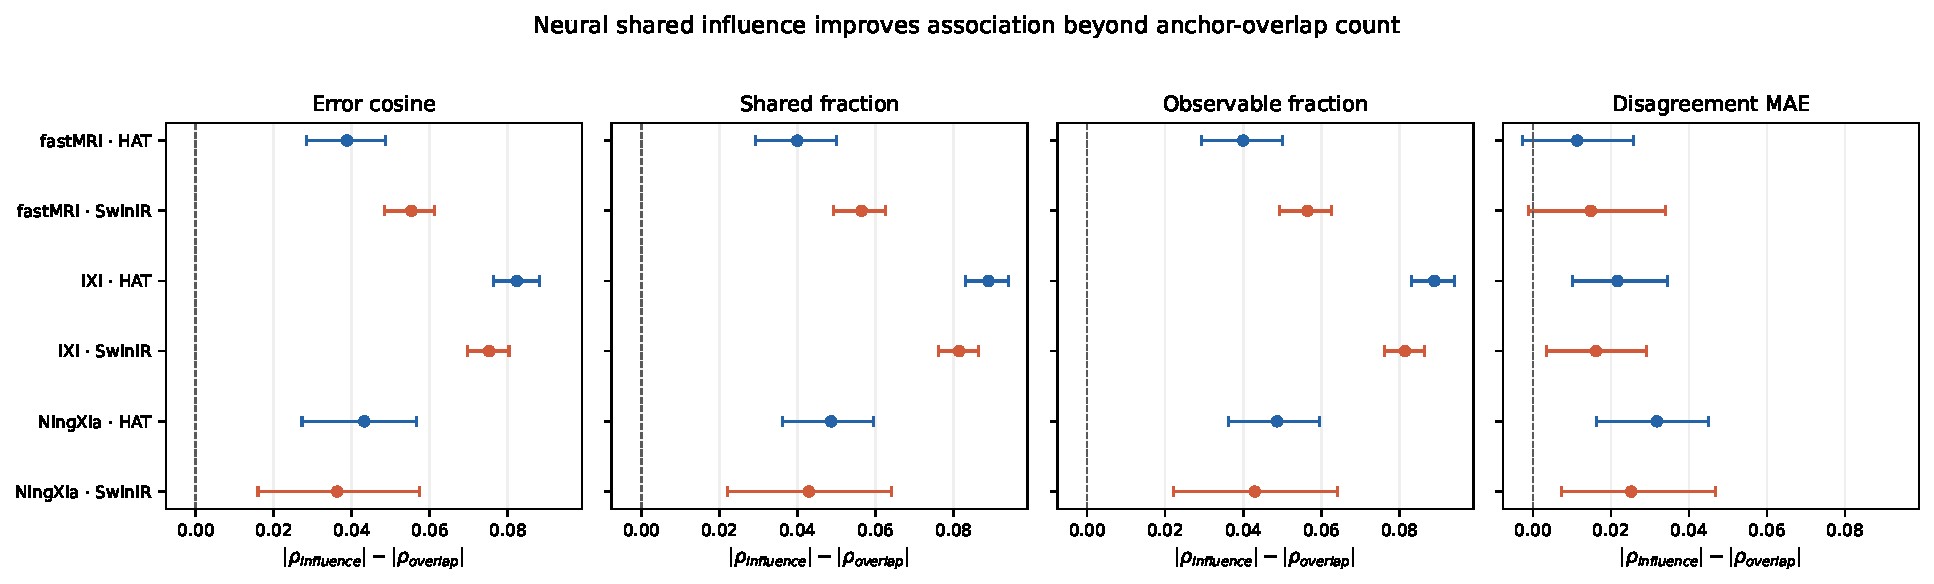
\includegraphics[width=\linewidth]{plan6_neural_influence_forest.pdf}
\caption{Clustered advantage of neural influence over overlap count. The supplement preserves endpoint/model strata rather than averaging them into one result.}
\label{fig:s_forest}
\end{figure}

\section{Exact Fixed-Count Test}
Table~\ref{tab:s_fixed} gives the strongest identifiable test beyond count: every comparison shares exactly one physical anchor. With count constant, the expected sign is positive for error cosine/shared fraction and negative for observable fraction/disagreement. All fastMRI and IXI intervals exclude zero. NingXia estimates are null or mixed, and every interval crosses zero. It is therefore incorrect to claim universal validation from all three cohorts; evidence beyond count is confirmed in the two larger cohorts and heterogeneous in the eight-patient cohort.

Holding the complete anchor-distance multiset fixed while changing overlap is combinatorially impossible with two physical inputs and a fixed target: changing which physical anchor is common necessarily changes at least one signed context assignment. The fixed-count design is the identifiable alternative because it removes the integer predictor and explicitly adjusts the remaining span/asymmetry variation.

\begin{table*}[t]
\centering
\caption{Partial Spearman association of neural influence at fixed overlap count $=1$. Brackets are clustered 95\% intervals.}
\label{tab:s_fixed}
\scriptsize
\setlength{\tabcolsep}{3.0pt}
\begin{tabular}{llcccc}
\toprule
Cohort&Model&Error cosine&Shared fraction&Observable fraction&Disagreement MAE\\
\midrule
fastMRI&HAT&.169 [.053,.283]&.135 [.023,.237]&$-.135$ [$-.243$,$-.024$]&$-.161$ [$-.276$,$-.055$]\\
&SwinIR&.350 [.212,.464]&.321 [.197,.425]&$-.321$ [$-.428$,$-.204$]&$-.286$ [$-.397$,$-.193$]\\
IXI&HAT&.346 [.259,.424]&.360 [.278,.437]&$-.360$ [$-.440$,$-.275$]&$-.543$ [$-.599$,$-.478$]\\
&SwinIR&.258 [.181,.335]&.241 [.168,.311]&$-.241$ [$-.311$,$-.168$]&$-.587$ [$-.636$,$-.529$]\\
NingXia&HAT&.014 [$-.232$,.223]&$-.006$ [$-.215$,.148]&.006 [$-.151$,.199]&$-.102$ [$-.218$,.116]\\
&SwinIR&$-.039$ [$-.175$,.144]&$-.039$ [$-.171$,.111]&.039 [$-.099$,.169]&$-.072$ [$-.151$,.057]\\
\bottomrule
\end{tabular}
\end{table*}

\section{Mechanism Chain, Arrow by Arrow}
Local arrows are estimated over plane--context observations, with uncertainty clustered at examination/patient. Arrow 1 is influence $\rightarrow$ error alignment conditional on geometry and examination. Arrow 2 is alignment $\rightarrow$ normalized disagreement conditional on influence and the same controls. Arrow 4a is influence $\rightarrow$ observable-error fraction. Every local estimate has the expected sign and interval excluding zero (Table~\ref{tab:s_chain}).

The final context-ranking arrow uses only eight non-self contexts per dataset/model. Greater alignment predicts worse disagreement--error ranking in all six point estimates, but intervals exclude zero only for both IXI architectures and NingXia HAT. Influence-to-ranking is weaker. These context summaries do not constitute a mediation analysis: sequential ignorability and a manipulable influence treatment are not established.

\begin{table*}[t]
\centering
\caption{Registered mechanism-chain estimates. Local arrows are partial $\rho$ with clustered 95\% intervals. Ranking is context-level Spearman; a dagger marks its interval excluding zero.}
\label{tab:s_chain}
\scriptsize
\setlength{\tabcolsep}{2.8pt}
\begin{tabular}{llcccc}
\toprule
Cohort&Model&Influence$\to$alignment&Alignment$\to$norm. disagreement&Influence$\to$observable&Alignment$\to$ranking\\
\midrule
fastMRI&HAT&.372 [.321,.428]&$-.926$ [$-.942$,$-.905$]&$-.370$ [$-.423$,$-.321$]&$-.143$\\
&SwinIR&.410 [.378,.441]&$-.933$ [$-.943$,$-.917$]&$-.412$ [$-.442$,$-.380$]&$-.333$\\
IXI&HAT&.347 [.321,.371]&$-.893$ [$-.909$,$-.874$]&$-.342$ [$-.366$,$-.315$]&$-.500^\dagger$\\
&SwinIR&.321 [.293,.347]&$-.890$ [$-.906$,$-.870$]&$-.298$ [$-.325$,$-.270$]&$-.643^\dagger$\\
NingXia&HAT&.258 [.173,.346]&$-.889$ [$-.920$,$-.857$]&$-.231$ [$-.295$,$-.171$]&$-.667^\dagger$\\
&SwinIR&.219 [.134,.310]&$-.898$ [$-.925$,$-.871$]&$-.211$ [$-.276$,$-.145$]&$-.548$\\
\bottomrule
\end{tabular}
\end{table*}

\section{Anchor-CV Identity and Explanation Audit}
ANCHOR\_CV\_V1 withholds each acquired interior $\times4$ anchor, predicts it by the midpoint of its two acquired neighbors, computes foreground MAE, and takes the examination median. Algebraically the residual is one half of the local second difference. Re-evaluation reproduced the stored scores to maximum absolute error $5.68\times10^{-14}$ after matching float32 masks.

The frozen x4-error Spearman correlations are .943/.955/.958 on fastMRI/IXI/NingXia. Adjacent-anchor MAE gives .934/.956/.973; adjacent RMSE gives .942/.956/.959. Clustered differences between Anchor-CV and adjacent MAE are .010 [$-.050$,.098], $-.001$ [$-.005$,.003], and $-.015$ [$-.133$,0]. Thus the trivial acquired baseline is statistically indistinguishable. The statement that leave-one-anchor reconstruction adds unavailable information is rejected.

\begin{table}[t]
\centering
\caption{Frozen Anchor-CV explanation audit.}
\label{tab:s_anchor}
\setlength{\tabcolsep}{3.2pt}
\begin{tabular}{lrrrr}
\toprule
Cohort&Anchor $\rho$&Adj. MAE $\rho$&Partial $\rho$&nAURC\\
\midrule
fastMRI&.943&.934&.333&.023\\
IXI&.955&.956&$-.059$&.015\\
NingXia&.958&.973&$-.100$&.011\\
\bottomrule
\end{tabular}
\end{table}

Partial $\rho$ conditions on adjacent MAE, robust intensity range, and through-plane spacing. Dividing Anchor-CV by robust intensity range lowers x4-error ranking from .943 to .455 on fastMRI, from .955 to $-.044$ on IXI, and from .958 to .736 on NingXia. Raw scale is therefore a material part of the useful examination ordering, not a nuisance that can be removed without consequence. Low-/high-frequency and gradient anchor differences also approach Anchor-CV on IXI; first-difference variability is consistently worse. No universal curvature or spectral explanation survives all cohorts.

\section{Architecture-Independent Examination Difficulty}
HAT--SwinIR case-error rank correlations are .989, 1.000, and .997. In a two-architecture squared-error decomposition, examination identity accounts for 99.1\%, 99.99\%, and 99.78\% on fastMRI/IXI/NingXia, while architecture after examination contributes .19\%, .004\%, and .029\%. The unusually strong performance of all simple acquired-data scores therefore occurs in a setting dominated by case difficulty rather than architecture choice.

Leave-one-examination/patient-cluster-out ridge using only Anchor-CV achieves $\rho=.939/.954/.953$ and held-out $R^2=.789/.900/.837$. Adding adjacent intensity/gradient/frequency differences, spacing, variability, and curvature does not improve ranks. On IXI, the direct and full blocks produce negative calibration $R^2$ ($-1.55$ and $-1.19$), a concrete failure of correlated feature stacking. No fusion score is promoted.

\section{Frozen Risk--Coverage and \texorpdfstring{$\times2$}{x2} Consequence}
Full risk--coverage curves retain cases from lowest predicted x4 risk upward. nAURC normalizes area between the method and oracle by the random--oracle area. Table~\ref{tab:s_risk} shows the complete architecture comparison. Output PC is strongest on fastMRI and IXI, whereas adjacent MAE is strongest on NingXia. Anchor-CV is useful but not superior.

\begin{table}[t]
\centering
\caption{Frozen x4 nAURC (lower is better).}
\label{tab:s_risk}
\setlength{\tabcolsep}{3.0pt}
\begin{tabular}{llrrr}
\toprule
Cohort&Model&Anchor&Adjacent&Output PC\\
\midrule
fastMRI&HAT&.0203&.0195&\textbf{.0154}\\
&SwinIR&.0314&.0240&\textbf{.0144}\\
IXI&HAT&.0149&.0144&\textbf{.0012}\\
&SwinIR&.0148&.0142&\textbf{.0012}\\
NingXia&HAT&.0094&\textbf{.0057}&.0135\\
&SwinIR&.0138&\textbf{.0100}&.0110\\
\bottomrule
\end{tabular}
\end{table}

\begin{figure}[t]
\centering
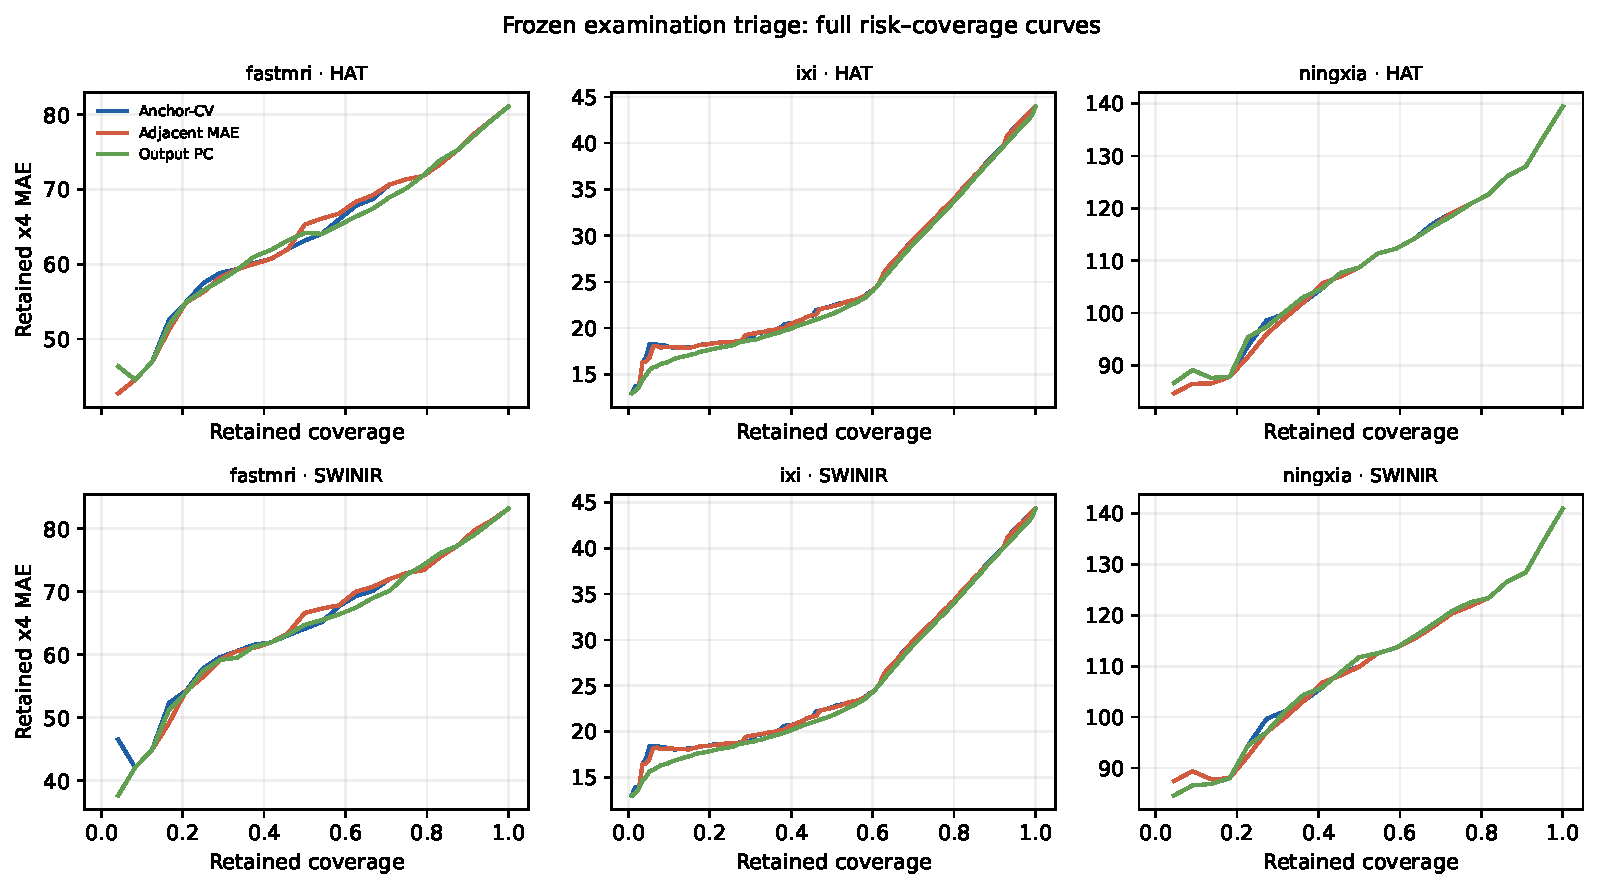
\includegraphics[width=\linewidth]{plan6_frozen_risk_coverage.pdf}
\caption{Every retained-case prefix in the frozen x4 risk audit. Curve crossings motivate reporting complete curves rather than one operating point.}
\label{fig:s_risk}
\end{figure}

For IXI $\times2$, the validation-selected I3Net checkpoint has SHA-256
\begin{center}\scriptsize\ttfamily
8C87AC897EBFD7C1\allowbreak66CB99F4A7B8922B\allowbreak FC4552BE79C242ABB\allowbreak39194C3DA21C3B8
\end{center}
Its 115 test predictions did not exist when the protocol was frozen. Benefit is mean HAT/SwinIR $\times4$ MAE minus frozen I3Net $\times2$ MAE. This cross-estimator endpoint asks whether a fixed score ranks realized case benefit; it does not isolate a same-model treatment effect.

Anchor/adjacent/PC benefit correlations are .871/.846/.843 on fastMRI and .948/.950/.970 on IXI. Table~\ref{tab:s_budget} reports all frozen budgets. Every clustered lower bound for gain above random is positive. No method dominates across dataset and budget.

\begin{table*}[t]
\centering
\caption{Selected mean $\times4\to\times2$ benefit minus random expectation. Parentheses give clustered 95\% intervals.}
\label{tab:s_budget}
\scriptsize
\setlength{\tabcolsep}{3.0pt}
\begin{tabular}{llcccc}
\toprule
Cohort&Method&10\%&20\%&30\%&50\%\\
\midrule
fastMRI&Anchor-CV&14.73 (7.14,19.28)&12.49 (5.21,15.89)&8.30 (4.19,11.94)&5.50 (2.86,7.72)\\
&Adjacent MAE&14.73 (6.37,19.03)&12.49 (4.67,15.95)&7.41 (3.32,11.95)&4.64 (2.40,7.38)\\
&Output PC&14.76 (8.81,19.84)&12.24 (7.59,16.33)&9.48 (5.08,12.27)&5.50 (2.56,7.96)\\
IXI&Anchor-CV&26.53 (20.67,33.82)&23.12 (19.88,27.34)&21.73 (18.69,24.32)&14.41 (12.13,16.66)\\
&Adjacent MAE&26.56 (20.81,33.29)&23.12 (19.71,27.17)&21.60 (18.42,24.05)&14.47 (12.05,16.64)\\
&Output PC&26.47 (20.95,33.44)&23.35 (19.65,27.26)&21.44 (18.76,24.37)&14.75 (12.55,16.80)\\
\bottomrule
\end{tabular}
\end{table*}

\begin{figure}[t]
\centering
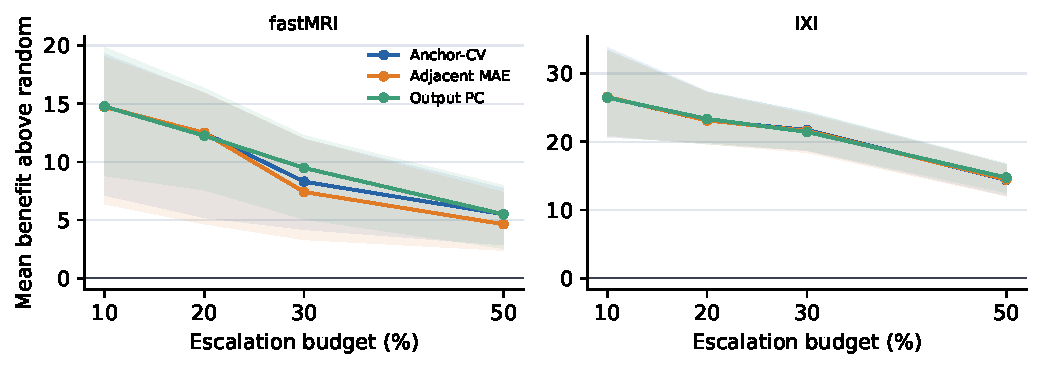
\includegraphics[width=\linewidth]{plan6_ixi_x2_budget.pdf}
\caption{Frozen retrospective allocation curves and clustered intervals. Scanner-time, motion, and clinical utility are not modeled.}
\label{fig:s_budget}
\end{figure}

\section{Failure Taxonomy and Granularity Boundary}
Using a frozen .20 absolute rank-error margin, output PC wins in three fastMRI and eight IXI architecture--cases; Anchor-CV wins in one fastMRI architecture--case. NingXia has no large-margin winner. The remaining 44/48 fastMRI, 222/230 IXI, and 44/44 NingXia architecture--cases are concordant. IXI PC-winner cases have lower adjacent difference and dynamic range than cohort medians, but eight cases are insufficient to define a transferable fusion rule.

Both scores are examination-level. Plane-level correlations can be weak or sign-inconsistent even when examination-level ordering is excellent. The qualitative panels in Fig.~\ref{fig:s_failures} therefore show the actual reconstruction and error map as well as the scalar score: neither scalar should be interpreted as a spatial failure detector.

\begin{figure}[t]
\centering
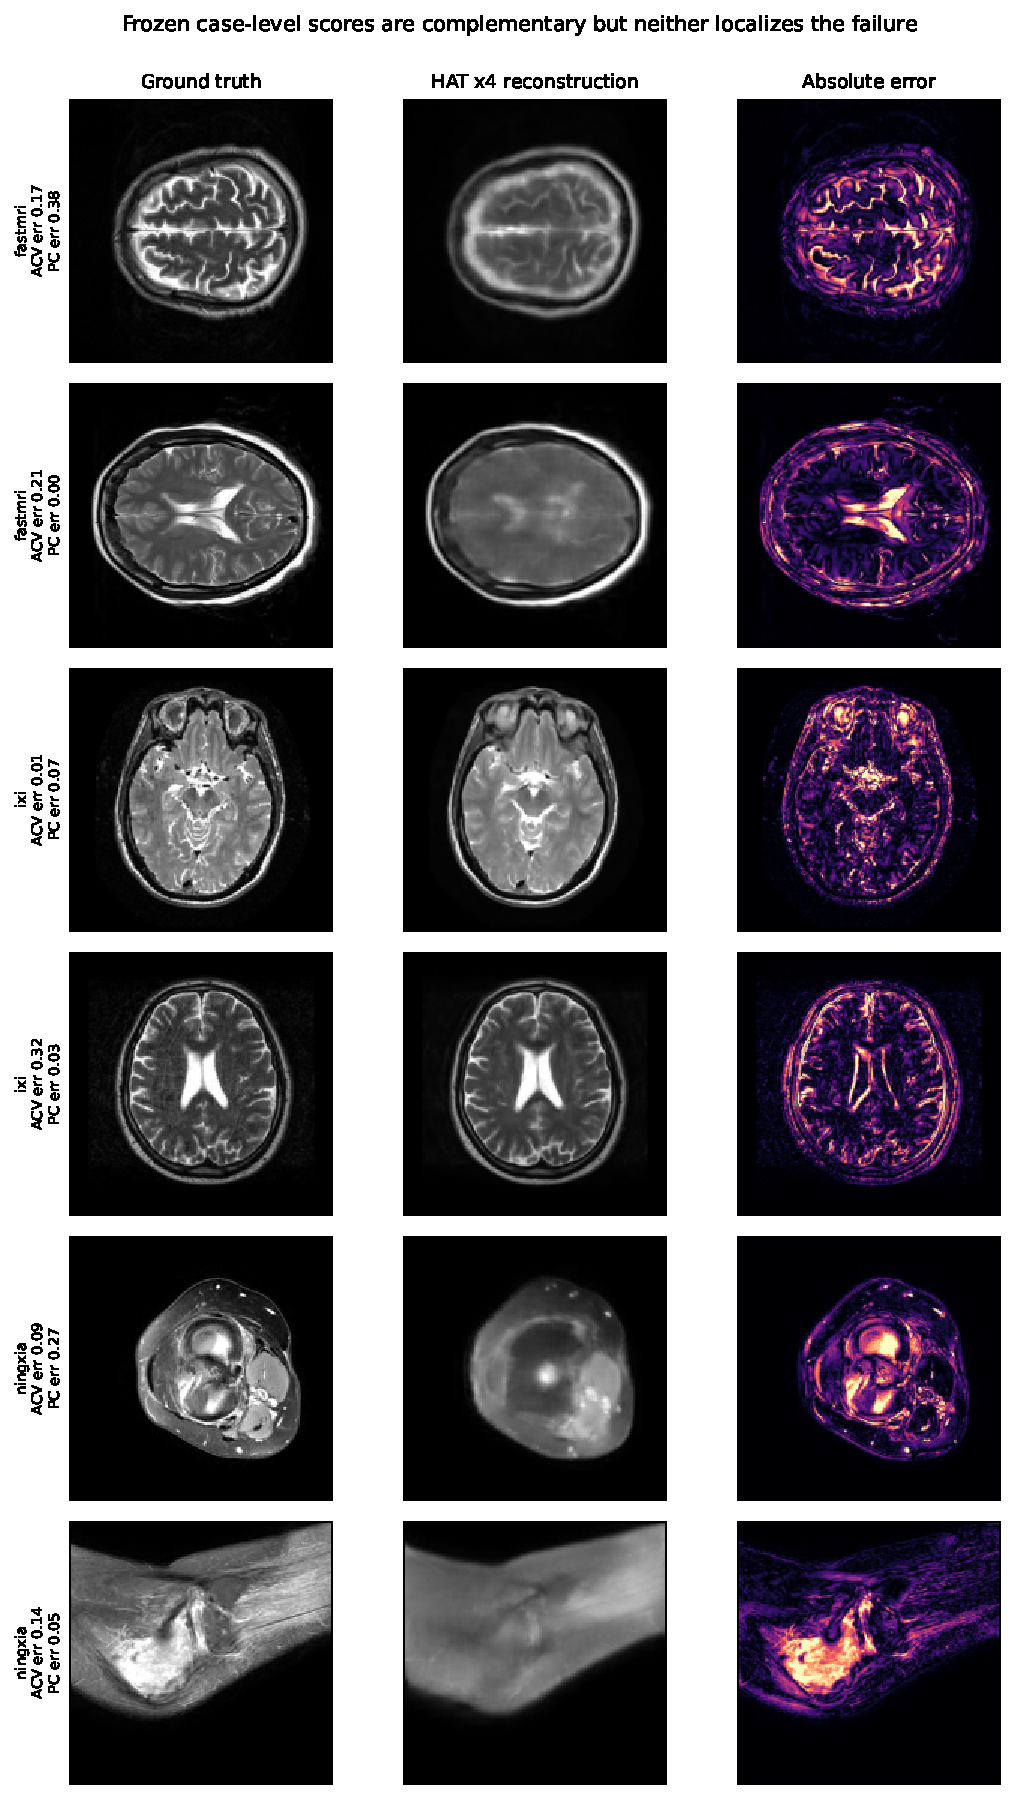
\includegraphics[width=\linewidth]{plan6_failure_exemplars.pdf}
\caption{Representative large-margin and granularity failures. Display windows are common within each row; error maps use a row-specific shared scale.}
\label{fig:s_failures}
\end{figure}

\section{Measured Computational Cost}
Measurements use deterministic median-index cases, an RTX 5090 D v2, three post-warm-up GPU repetitions, and 100 CPU score repetitions. Neural-call times are sequential totals. Peak memory is peak allocated GPU memory, not reserved memory. Stored output is the uncompressed float32 volume pair required by the score.

\begin{table*}[t]
\centering
\caption{Representative end-to-end strategy cost. Output PC score-only latency excludes generation of its two required predictions.}
\label{tab:s_cost}
\setlength{\tabcolsep}{4.0pt}
\begin{tabular}{llrrrr}
\toprule
Cohort&Strategy&Neural calls&Median time&Peak MiB&Stored MiB\\
\midrule
fastMRI&Anchor-CV&0&0.42 ms&0&0\\
&Committee / flip-TTA / disjoint&2&0.25 / 0.26 / 0.29 s&271&10.2 / 10.2 / 8.6\\
IXI&Anchor-CV&0&3.97 ms&0&0\\
&Committee / flip-TTA / disjoint&2&2.43 / 3.18 / 3.20 s&271&66.5 / 66.5 / 65.5\\
NingXia&Anchor-CV&0&3.93 ms&0&0\\
&Committee / flip-TTA / disjoint&2&0.49 / 0.60 / 0.56 s&271&36.2 / 36.2 / 31.9\\
\bottomrule
\end{tabular}
\end{table*}

The operational conclusion is narrow. Anchor-CV is cheap because it runs on acquired anchors, not because it is more accurate. Adjacent difference is equally reconstruction-free and statistically competitive. Output PC can be preferable when two reconstructions already exist, but its apparent score-only speed would be misleading if prediction generation were omitted.

\section{Plan7 Locked Method Gates}
\label{sec:p7-gates}
Plan7 asked whether shared influence yields information unavailable from adjacent-anchor difference or ordinary output disagreement. Three rules were specified without evaluation-label tuning. None passed the promotion gate, and no failed rule was reweighted on transfer cohorts.

\paragraph{Minimum-influence context selection (P7-CV-E01).}
Four candidate contexts each share exactly one anchor with reference $(-2,+2)$. The rule selects the context with minimum neural influence; target error never enters selection. Development and confirmation are the first/last 12 fastMRI examinations; IXI and NingXia are untouched transfers. On fastMRI confirmation, selected-score Spearman was $.986/.965$ for HAT/SwinIR. On IXI it was $.973/.977$, below random-context expectation $.983/.983$ and output PC $.994/.994$; the selected-minus-PC clustered intervals were entirely below zero. NingXia estimates were $.957/.940$ versus random $.980/.958$ and adjacent MAE $.976/.971$, with eight-patient intervals too wide for a transferable gain. Neural influence is also identically zero when no physical anchor is shared, so the statistic cannot rank zero-overlap candidates.

\paragraph{Multi-anchor jackknife (P7-CV-E03).}
For each internal acquired anchor we compute a pseudo-target residual from complementary acquired contexts. Development-only selection chose residual IQR from the prespecified location/dispersion family. It ranked error at $.629$ on fastMRI development but only $.399$ on confirmation, versus $.944$ for adjacent MAE (delta $-.545$, clustered 95\% interval $[-1.138,-.143]$). Transfer correlations were $.732$ versus $.956$ on IXI and $.310$ versus $.973$ on NingXia; conditional associations beyond adjacent change, scale and spacing were negative or uncertain.

\paragraph{Covariance-derived residualization (P7-CV-E04).}
With zero fitted parameters, each context disagreement $d$ is corrected as $d/\sqrt{1-\min(I,.95)}$ and aggregated by the median. On fastMRI confirmation it tied raw disagreement for HAT and decreased Spearman by $.014$ for SwinIR. IXI changes were only $+.0011/+.0006$, both with clustered intervals crossing zero. NingXia changed by $-.0011/+.0068$ with wide intervals. Thus a covariance identity does not create a useful ranking correction by itself.

\begin{table*}[t]
\centering
\caption{Locked Plan7 capability tests. Values are Spearman correlations with examination error; development is shown only where it selected a statistic.}
\label{tab:s_p7_gates}
\setlength{\tabcolsep}{4pt}
\begin{tabular}{llrrrrrr}
\toprule
Branch&Partition&\multicolumn{2}{c}{fastMRI}&\multicolumn{2}{c}{IXI}&\multicolumn{2}{c}{NingXia}\\
&&HAT&SwinIR&HAT&SwinIR&HAT&SwinIR\\
\midrule
Minimum influence&confirmation/transfer&.986&.965&.973&.977&.957&.940\\
Random expectation&confirmation/transfer&.965&.944&.983&.983&.980&.958\\
Output PC&confirmation/transfer&.979&.958&.994&.994&.951&.941\\
Residualized disagreement&confirmation/transfer&.965&.944&.986&.986&.948&.955\\
Raw disagreement&confirmation/transfer&.965&.958&.985&.985&.949&.948\\
\bottomrule
\end{tabular}
\end{table*}

The method gate required mechanistic necessity, non-triviality beyond simple scores, locked evidence, multi-stratum robustness, deployment-time information and a genuinely new capability. Local fastMRI success cannot compensate for transfer failure; all three branches remain negative evidence rather than contributions disguised by post-hoc tuning.

\section{Prespecified Neural-Influence Stability Audit}
P7-CV-E02 freezes baseline Rademacher positive perturbations at 1\% amplitude with four directions. It varies amplitude (0.5/1/2\%), sign, Rademacher versus Gaussian field, and 1/2/4/8 directions on the full central-plane cohorts for HAT and SwinIR. For each nonbaseline condition, rank stability versus baseline must be at least $.85$ in five of six dataset--architecture strata and no stratum may fall below $.70$. The same gate is applied to each pair among three frozen physical planes.

All seven perturbation conditions pass in all six strata, stronger than the registered gate: minima are $.948$ (Gaussian field), $.973$ (negative sign), $.949$ (0.5\% amplitude), $.942$ (one direction), $.972$ (two directions), $.991$ (eight directions), and $.960$ (2\% amplitude). Associations with error cosine/shared fraction retain the expected sign in every condition. Thus the central-plane estimate is not a single-seed, amplitude, sign, or field artifact.

Plane choice is less stable. For early--central, early--late and central--late plane pairs, stability spans $.794$--$.953$, $.779$--$.887$ and $.856$--$.934$, respectively. Only central--late passes in all six strata; the other pairs have four and three strata at or above $.85$. Each plane separately retains the expected association sign, but context ranks are not plane-invariant. We therefore reject the broad stability hypothesis and retain a narrower statement: perturbation parameters are robust at a declared local plane, while physical plane is a material analysis choice.

\begin{table}[t]
\centering
\caption{P7-CV-E02 stability gates across six dataset--architecture strata.}
\label{tab:s_stability}
\resizebox{\columnwidth}{!}{%
\begin{tabular}{lrrl}
\toprule
Condition family&Minimum $\rho$&Strata $\geq.85$&Gate\\
\midrule
Amplitude/sign/field/directions&.942&42/42&Pass\\
Plane pair 1--2&.794&4/6&Fail\\
Plane pair 1--3&.779&3/6&Fail\\
Plane pair 2--3&.856&6/6&Pass\\
\bottomrule
\end{tabular}
}
\end{table}

\section{Prespecified and Material Negative Results}
\label{sec:negative}
\begin{enumerate}
\item Integer overlap is not a monotone causal dose. The exact analytical ladder reverses at $0\to1$ in every compact cohort and in the wider IXI replication.
\item Fixed-count neural influence does not confirm on NingXia: all intervals cross zero and some point estimates reverse.
\item The full ranking chain is not uniformly supported. Local cancellation arrows are strong, but context-level ranking has only eight configurations and three of six intervals cross zero.
\item Anchor-CV is not uniquely informative. Adjacent MAE/RMSE are statistically indistinguishable and partial association vanishes on IXI/NingXia.
\item Scale normalization does not isolate a cleaner invariant score; it substantially harms ranking and reverses IXI.
\item Naive feature fusion fails. The all-acquired block harms IXI held-out calibration and does not improve ranks.
\item Anchor-CV and PC do not localize the worst physical plane. Their supported use is examination triage.
\item No score dominates frozen risk curves or benefit budgets. The preferred score depends on what outputs already exist and on cohort/budget.
\item The $\times2$ consequence evidence is retrospective. It neither optimizes prospective acquisition nor models scanner-time and clinical costs.
\item Minimum-influence context selection succeeds locally on fastMRI but transfers below random expectation/output PC on IXI and is heterogeneous on NingXia.
\item Multi-anchor jackknife IQR and covariance-derived influence residualization fail locked non-triviality and transfer gates.
\item Finite-difference rankings are robust to the tested perturbation parameters but not invariant to physical plane; two of three plane-pair gates fail.
\end{enumerate}

\section{Reproducibility and Evidence Map}
All artifacts are under \texttt{CVPR/CVPR\_UPGRADE/}. The three-cohort manifest is \texttt{DATA\_MANIFEST.csv}. Registered hypotheses and decision rules are in \texttt{HYPOTHESES.md} and \texttt{EXPERIMENTS.md}. The main machine-readable outputs are:
\begin{itemize}
\item neural influence: \path{outputs/plan6_neural_shared_influence_confirm3*};
\item fixed-count test: \path{outputs/plan6_fixed_overlap_ladder.*};
\item chain: \path{outputs/plan6_mechanism_chain*};
\item Anchor-CV audit: \path{outputs/plan6_anchor_cv_explanation*};
\item difficulty/failures/cost: \path{outputs/plan6_intrinsic_difficulty*}, \path{plan6_failure_taxonomy*}, and \path{plan6_efficiency.*};
\item risk and consequence: \path{outputs/plan6_frozen_risk_coverage*} and \path{plan6_ixi_x2_consequence*}.
\item Plan7 gates: \path{../../PLAN7_ACCEPTANCE_OPTIMIZATION/outputs/p7_cvpr_influence_context_selection*}, \path{p7_cvpr_multi_anchor_jackknife*}, and \path{p7_cvpr_influence_residualization*}.
\item stability: \path{../../PLAN7_ACCEPTANCE_OPTIMIZATION/outputs/p7_cvpr_neural_influence_stability*} and \path{p7_cvpr_neural_influence_plane_rank_stability.csv}.
\end{itemize}
Scripts in \texttt{scripts/} have matching Plan6 prefixes. Submission figures \texttt{plan6\_anchor\_cv\_audit} and \texttt{plan6\_ixi\_x2\_budget} are generated directly from the frozen CSV tables by \texttt{scripts/plan6\_make\_submission\_figures.py}. This mapping is intended for internal artifact verification; the review PDF itself is self-contained and does not rely on external links.

\end{document}
